%==============================================================
%  EE201 -- Circuit Theory I
%  Lecture 15 : Nonlinear Resistive Circuits
%  M. Mert Ankaralı, METU EEE
%
%  Compile:  ./build.sh      (or: pdflatex EE201_Lecture_15.tex, twice)
%==============================================================
\documentclass[11pt,a4paper]{article}

%-------------------- packages --------------------------------
\usepackage[T1]{fontenc}
\usepackage[utf8]{inputenc}
\usepackage[english]{babel}
\usepackage{lmodern}
\usepackage[margin=2.3cm,top=2.0cm,bottom=1.9cm,headheight=14pt,headsep=9pt]{geometry}
\usepackage{amsmath,amssymb}
\usepackage{array,booktabs,tabularx}
\usepackage{enumitem}
\usepackage{needspace}
\usepackage[table]{xcolor}
\usepackage{fancyhdr}
\usepackage{titlesec}
\usepackage{graphicx}
\usepackage[most]{tcolorbox}
\usepackage{tikz}
\usepackage[american,siunitx]{circuitikz}
\usetikzlibrary{matrix,arrows.meta,positioning,calc,decorations.pathmorphing,decorations.pathreplacing,decorations.markings,patterns,shapes.geometric}
\usepackage[colorlinks=true,allcolors=metured,breaklinks=true]{hyperref}

%-------------------- colour system ---------------------------
% One colour per physical quantity, used identically in the slides.
\definecolor{metured}{RGB}{155,27,48}    % headings, structure
\definecolor{metugray}{RGB}{88,89,91}
\definecolor{ccur}{RGB}{0,102,170}       % CURRENT  -- blue
\definecolor{cvolt}{RGB}{214,120,0}      % VOLTAGE  -- orange
\definecolor{cpow}{RGB}{23,128,74}       % POWER / ENERGY -- green
\definecolor{ccharge}{RGB}{124,60,160}   % CHARGE   -- purple
\definecolor{cflux}{RGB}{0,138,138}      % FLUX -- teal
\definecolor{boxgray}{RGB}{245,245,245}
\definecolor{copper}{RGB}{184,98,30}

\newcommand{\Icol}[1]{\textcolor{ccur}{#1}}
\newcommand{\Vcol}[1]{\textcolor{cvolt}{#1}}
\newcommand{\Pcol}[1]{\textcolor{cpow}{#1}}
\newcommand{\Qcol}[1]{\textcolor{ccharge}{#1}}
\newcommand{\Fcol}[1]{\textcolor{cflux}{#1}}

%-------------------- units (no siunitx dependency) -----------
\newcommand{\uni}[1]{\,\mathrm{#1}}
\newcommand{\A}{\uni{A}}   \newcommand{\V}{\uni{V}}
\newcommand{\W}{\uni{W}}   \newcommand{\J}{\uni{J}}
\newcommand{\Cb}{\uni{C}}  \newcommand{\s}{\uni{s}}
\newcommand{\Sie}{\uni{S}} \newcommand{\Wb}{\uni{Wb}}

%-------------------- layout ----------------------------------
\pagestyle{fancy}
\fancyhf{}
\lhead{\small\textcolor{metugray}{EE201 -- Circuit Theory I}}
\rhead{\small\textcolor{metugray}{Lecture 15: Nonlinear Resistive Circuits}}
\cfoot{\small\thepage}
\renewcommand{\headrulewidth}{0.4pt}

\titleformat{\section}{\large\bfseries\color{metured}}{\thesection.}{0.6em}{}
\titleformat{\subsection}{\normalsize\bfseries\color{metugray}}{\thesubsection.}{0.6em}{}
\titlespacing*{\section}{0pt}{1.4ex plus .3ex}{0.7ex}
\titlespacing*{\subsection}{0pt}{1.1ex plus .2ex}{0.5ex}

\setlist[itemize]{itemsep=2pt,topsep=3pt,parsep=0pt,leftmargin=1.5em}
\setlist[enumerate]{itemsep=2pt,topsep=3pt,parsep=0pt,leftmargin=1.7em}
\setlength{\parindent}{0pt}
\setlength{\parskip}{0.7ex plus .1ex}
\raggedbottom
\widowpenalty=10000
\clubpenalty=10000
\brokenpenalty=10000

%-------------------- boxes -----------------------------------
\newtcolorbox{definitionbox}[1]{enhanced,
  colback=metured!4, colframe=metured, boxrule=0.9pt,
  fonttitle=\bfseries, title={#1}, arc=2pt,
  left=7pt,right=7pt,top=5pt,bottom=5pt, before skip=7pt, after skip=7pt,
  before upper={\setlength{\parskip}{0.6ex plus .1ex}}}

\newtcolorbox{ideabox}[1][Key idea]{enhanced,
  colback=ccur!5, colframe=ccur, boxrule=0.9pt,
  fonttitle=\bfseries, title={#1}, arc=2pt,
  left=7pt,right=7pt,top=5pt,bottom=5pt, before skip=7pt, after skip=7pt,
  before upper={\setlength{\parskip}{0.6ex plus .1ex}}}

\newtcolorbox{examplebox}[1][Example]{enhanced,
  colback=cpow!4, colframe=cpow, boxrule=0.9pt,
  fonttitle=\bfseries, title={#1}, arc=2pt,
  left=7pt,right=7pt,top=5pt,bottom=5pt, before skip=7pt, after skip=7pt,
  before upper={\setlength{\parskip}{0.6ex plus .1ex}}}

%  Example solutions: a heading and numbered steps outside the example box
\newif\ifsolfirst
\newcommand{\solution}{\par\smallskip\noindent{\color{cpow}\bfseries Solution}\par\nobreak\smallskip\global\solfirsttrue}
\newcommand{\solstep}[2]{\par\ifsolfirst\global\solfirstfalse\else\medskip\needspace{5\baselineskip}\fi
  \noindent{\color{cpow}\bfseries Step #1.}\ {\bfseries #2}\par\nobreak\smallskip}

\newtcolorbox{cautionbox}[1][Careful]{enhanced,
  colback=cvolt!6, colframe=cvolt, boxrule=0.9pt,
  fonttitle=\bfseries, title={#1}, arc=2pt,
  left=7pt,right=7pt,top=5pt,bottom=5pt, before skip=7pt, after skip=7pt,
  before upper={\setlength{\parskip}{0.6ex plus .1ex}}}

%-------------------- circuitikz defaults ---------------------
%  voltage sources: smaller + and - inside the circle, further apart
\ctikzset{bipoles/vsourceam/inner plus={\tiny$+$},
          bipoles/vsourceam/inner minus={\tiny$\vphantom{+}-$},
          bipoles/vsourceam/margin=0.85,
          bipoles/cvsourceam/inner plus={\tiny$+$},
          bipoles/cvsourceam/inner minus={\tiny$\vphantom{+}-$},
          bipoles/cvsourceam/margin=0.85}
\ctikzset{bipoles/length=0.9cm, color=black,
          label/align=straight,
          bipoles/generic/height=0.28, bipoles/generic/width=0.62}
\tikzset{
  iar/.style={-{Stealth[length=2.2mm]}, ccur, thick},
  pol/.style={font=\small, text=cvolt},
  glab/.style={font=\footnotesize, text=metured},
  ttl/.style={font=\scriptsize\bfseries, text=metugray},
  capn/.style={font=\scriptsize, text=metugray, align=center},
  bigarr/.style={-{Stealth[length=3mm]}, very thick, metugray},
  gnode/.style={circle, fill=metured, inner sep=0pt, minimum size=4.4pt},
  nlab/.style={circle, draw=metured, text=metured, font=\scriptsize, inner sep=0.7pt},
  blab/.style={font=\footnotesize, text=black!80},
  gbr/.style={black!75, thick, postaction={decorate, decoration={markings,
      mark=at position 0.56 with {\arrow{Stealth[length=2.5mm]}}}}},
  apbr/.style={ccur, line width=1.7pt, postaction={decorate, decoration={markings,
      mark=at position 0.56 with {\arrow{Stealth[length=2.8mm]}}}}},
  hal/.style={draw=cpow!60, line width=6pt, opacity=0.35, line cap=round, line join=round},
  elem/.style={draw=metugray, thick, fill=metulight},
}
\definecolor{metulight}{RGB}{243,240,241}

%-------------------- Lecture 15 circuit macros ---------------
\newcommand{\ohm}{\,\Omega}
\newcommand{\yes}{\textcolor{cpow}{\checkmark}}
\newcommand{\e}[1]{\textcolor{cvolt}{e_{#1}}}
\newcommand{\gnd}[2]{\draw (#1,#2) -- ++(0,-0.2) node[ground] {};}
\newcommand{\Rth}{R_{\mathrm{th}}}
\newcommand{\vth}{\Vcol{v_{\mathrm{th}}}}
\newcommand{\voc}{\Vcol{v_{\mathrm{oc}}}}
%  Labels beside a vertical element at (#1,#2), a fixed distance to the right (\lR) or left (\lL)
\newcommand{\lR}[3]{\node[anchor=west, xshift=7pt, font=\small] at (#1,#2) {#3};}
\newcommand{\lL}[3]{\node[anchor=east, xshift=-7pt, font=\small] at (#1,#2) {#3};}
\tikzset{tlab/.style={font=\small\bfseries, text=black!80},
         vax/.style={-{Stealth[length=2mm]}, gray!70},
         crv/.style={metured, very thick, line join=round},
         crvb/.style={ccur, very thick, line join=round},
         lline/.style={ccur, thick, dashed},
         opt/.style={circle, fill=black, inner sep=0pt, minimum size=5pt}}

%  v-i axes: x from -#1 to #1, y from -#2 to #2 (v horizontal, i vertical), #3 = caption below
\newcommand{\ivax}[3]{%
  \draw[vax] (-#1,0) -- (#1,0) node[right=1pt, font=\scriptsize, text=cvolt] {$v$};
  \draw[vax] (0,-#2) -- (0,#2) node[above=1pt, font=\scriptsize, text=ccur] {$i$};
  \node[font=\scriptsize, text=metugray] at (0,-#2-0.35) {#3};}
%  First-quadrant axes: x to #1, y to #2
\newcommand{\ivq}[2]{%
  \draw[vax] (-0.2,0) -- (#1,0) node[right=1pt, font=\scriptsize, text=cvolt] {$v$};
  \draw[vax] (0,-0.2) -- (0,#2) node[above=1pt, font=\scriptsize, text=ccur] {$i$};}

%  Terminal pair at x = #1 (top y = #2, bottom 0): i into the top terminal, + v - beside it
\newcommand{\tpair}[2]{%
  \draw (#1,#2) node[ocirc] {}; \draw (#1,0) node[ocirc] {};
  \draw[iar] (#1-0.65,#2) -- (#1-0.15,#2);
  \node[font=\small, text=ccur] at (#1-0.4,#2+0.3) {$i$};
  \node[pol] at (#1-0.35,0.72*#2) {$+$}; \node[pol] at (#1-0.35,0.22*#2) {$-$};
  \node[font=\small, text=cvolt] at (#1-0.35,0.47*#2) {$v$};}

%  A source E, a resistor R and one nonlinear resistor; #1 = E label, #2 = R label
\newcommand{\nlone}[2]{%
  \draw (0,2) to[american voltage source, l_=#1] (0,0);
  \draw (0,2) to[R, l=#2] (2.4,2);
  \draw (2.4,2) to[generic] (2.4,0) -- (0,0);
  \draw[iar] (2.75,1.55) -- (2.75,0.95); \node[font=\small, text=ccur, anchor=west] at (2.8,1.25) {$i$};
  \node[pol] at (2.05,1.55) {$+$}; \node[pol] at (2.05,0.45) {$-$};
  \node[font=\small, text=cvolt] at (2.0,1.0) {$v$};}

%  A nonlinear resistor at port a-b of a linear circuit (#1 = 0) or of its Thevenin equivalent (#1 = 1)
\newcommand{\nlport}[1]{%
  \ifcase#1
    \draw[thick, fill=gray!8] (0,0) rectangle (2.6,2.4);
    \node[font=\small\bfseries] at (1.3,1.5) {linear};
    \node[font=\scriptsize, align=center] at (1.3,0.9) {resistors,\\ sources};
    \draw (2.6,2.0) -- (3.3,2.0); \draw (2.6,0.4) -- (3.3,0.4);
  \or
    \draw (0.4,2.0) to[R, l=$\Rth$] (2.0,2.0) -- (3.3,2.0);
    \draw (0.4,2.0) to[american voltage source, l_=$\vth$] (0.4,0.4);
    \draw (0.4,0.4) -- (3.3,0.4);
  \fi
  \draw (3.3,2.0) -- (4.2,2.0) to[generic] (4.2,0.4) -- (3.3,0.4);
  \draw (3.3,2.0) node[ocirc] {}; \draw (3.3,0.4) node[ocirc] {};
  \node[font=\small, anchor=south] at (3.3,2.05) {a}; \node[font=\small, anchor=north] at (3.3,0.35) {b};
  \node[pol] at (3.75,1.75) {$+$}; \node[pol] at (3.75,0.65) {$-$};
  \node[font=\small, text=cvolt] at (3.72,1.2) {$v_R$};
  \draw[iar] (4.6,1.55) -- (4.6,0.95); \node[font=\small, text=ccur, anchor=west] at (4.65,1.25) {$i_R$};
  \node[font=\scriptsize, text=metured, anchor=west] at (4.45,2.1) {nonlinear};}

%  The load line picture: a bent curve, the line R i + v = E, the operating point
\newcommand{\loadpic}{%
  \ivq{5.4}{2.7}
  \draw[crv, domain=0:1.12, samples=60, smooth] plot (\x,{2*\x*\x});
  \node[font=\scriptsize, text=metured, anchor=west] at (1.35,2.4) {$i = g(v)$};
  \draw[lline] (0,2.0) -- (5.0,0);
  \node[font=\scriptsize, text=ccur, anchor=west] at (3.2,1.05) {load line $R\,i + v = E$};
  \node[font=\scriptsize, left] at (0,2.0) {$E/R$};
  \node[font=\scriptsize, below] at (5.0,0) {$E$};
  \node[opt] at (0.905,1.638) {};
  \draw[dotted, gray] (0.905,0) -- (0.905,1.638) -- (0,1.638);
  \node[font=\scriptsize, below] at (0.905,0) {$v_o$};
  \node[font=\scriptsize, left] at (0,1.638) {$i_o$};
  \node[font=\scriptsize, anchor=west] at (1.05,1.9) {operating point};}

%  Example 15.1: v from 0 to 10 V (x = v/2), i from 0 to 0.12 A (y = 20 i)
\newcommand{\exOnePlot}{%
  \ivq{5.6}{2.6}
  \draw[crv, domain=0:1.0, samples=60, smooth] plot (\x,{2.4*\x*\x});
  \draw[crv] (-0.2,0) -- (0,0);
  \node[font=\scriptsize, text=metured] at (1.45,2.35) {$i = \tfrac{3}{100}\,v^2$};
  \draw[lline] (0,2.0) -- (5.0,0);
  \node[font=\scriptsize, left] at (0,2.0) {$0.1\A$};
  \node[font=\scriptsize, below] at (5.0,0) {$10\V$};
  \node[opt] at (0.833,1.667) {};
  \draw[dotted, gray] (0.833,0) -- (0.833,1.667);
  \node[font=\scriptsize, below] at (0.833,0) {$\tfrac53\V$};}

%  Many or no operating points
\newcommand{\manypic}{%
  \ivq{5.2}{2.6}
  \draw[crv, domain=0:4.6, samples=90, smooth] plot (\x,{1.4 - 0.25*\x + 0.239*(\x-0.7)*(\x-2.2)*(\x-3.8)});
  \draw[lline] (0,1.4) -- (4.9,0.175);
  \foreach \x in {0.7,2.2,3.8} \node[opt] at (\x,{1.4-0.25*\x}) {};}
\newcommand{\nonepic}{%
  \ivq{5.2}{2.6}
  \draw[crv, domain=0.5:5.0, samples=60, smooth] plot (\x,{1.25/\x});
  \node[font=\scriptsize, text=metured] at (4.1,0.6) {$v\,i = P$};
  \draw[lline] (0,1.2) -- (3.0,0);}

%  Example 15.2: 7.2 V, 6 Ohm, 12 Ohm (voltage v), 4 Ohm, 8 Ohm, nonlinear resistor at a.
%  #1 = 0: the circuit;  1: nonlinear resistor removed (port a-b);  2: replaced by 2 V
\newcommand{\exTwo}[1]{%
  \draw (0,0) to[american voltage source, invert, l=$\Vcol{7.2\V}$] (0,2.2);
  \draw (0,2.2) to[R, l=$6\ohm$] (2.2,2.2) to[R, l=$4\ohm$] (4.4,2.2);
  \draw (0,2.2) -- (0,3.2) to[R, l=$8\ohm$] (4.4,3.2) -- (4.4,2.2);
  \draw (2.2,2.2) to[R] (2.2,0); \lL{2.2}{1.1}{$12\ohm$}
  \node[pol] at (2.55,1.6) {$+$}; \node[pol] at (2.55,0.55) {$-$};
  \node[font=\small, text=cvolt] at (2.6,1.07) {$v$};
  \draw (0,0) -- (4.4,0);
  \fill (2.2,2.2) circle (1.7pt); \fill (2.2,0) circle (1.7pt); \fill (0,2.2) circle (1.7pt);
  \ifcase#1
    \draw (4.4,2.2) to[generic] (4.4,0);
    \draw[iar] (4.75,1.55) -- (4.75,0.95); \node[font=\small, text=ccur, anchor=west] at (4.8,1.25) {$i_R$};
    \node[pol] at (4.05,1.55) {$+$}; \node[pol] at (4.05,0.45) {$-$};
    \node[font=\small, text=cvolt] at (3.98,1.0) {$v_R$};
    \fill (4.4,2.2) circle (1.7pt); \fill (4.4,0) circle (1.7pt);
  \or
    \draw (4.4,2.2) -- (5.4,2.2) node[ocirc] {} node[above, tlab] {a};
    \draw (4.4,0) -- (5.4,0) node[ocirc] {} node[below, tlab] {b};
    \fill (4.4,2.2) circle (1.7pt);
  \or
    \draw (4.4,0) to[american voltage source, invert, l_=$\Vcol{2\V}$] (4.4,2.2);
    \fill (4.4,2.2) circle (1.7pt); \fill (4.4,0) circle (1.7pt);
    \node[font=\small, text=cvolt, above] at (2.2,2.25) {$e$};
    \gnd{1.1}{0}
  \fi}
%  Example 15.2: the Thevenin equivalent with the nonlinear resistor
\newcommand{\exTwoTh}{%
  \draw (0,0) to[american voltage source, invert, l=$\Vcol{6\V}$] (0,2);
  \draw (0,2) to[R, l=$4\ohm$] (2.4,2);
  \draw (2.4,2) to[generic] (2.4,0) -- (0,0);
  \draw[iar] (2.75,1.55) -- (2.75,0.95); \node[font=\small, text=ccur, anchor=west] at (2.8,1.25) {$i_R$};
  \node[pol] at (2.05,1.55) {$+$}; \node[pol] at (2.05,0.45) {$-$};
  \node[font=\small, text=cvolt] at (1.98,1.0) {$v_R$};}
%  Example 15.2 plot: v from 0 to 6 V (x = 0.8 v), i from 0 to 1.5 A (y = 1.5 i)
\newcommand{\exTwoPlot}{%
  \ivq{5.4}{2.7}
  \draw[crv, domain=0:1.95, samples=60, smooth] plot (\x,{0.586*\x*\x});
  \node[font=\scriptsize, text=metured] at (2.55,2.5) {$i_R = \tfrac14\,v_R^2$};
  \draw[lline] (0,2.25) -- (4.8,0);
  \node[font=\scriptsize, left] at (0,2.25) {$1.5\A$};
  \node[font=\scriptsize, below] at (4.8,0) {$6\V$};
  \node[opt] at (1.6,1.5) {};
  \draw[dotted, gray] (1.6,0) -- (1.6,1.5) -- (0,1.5);
  \node[font=\scriptsize, below] at (1.6,0) {$2\V$};
  \node[font=\scriptsize, left] at (0,1.5) {$1\A$};}

%-------------------- the ideal diode and piecewise-linear pieces ---------------
%  A vertical two-terminal branch from (x,#2) down to (x,0) drawn by #3, with i, + v -
%  Plot curves (axes half-widths 1.3 x 1.1). Each curve in red, drawn over the axes.
\newcommand{\pD}{\draw[crv] (-1.2,0) -- (0,0) -- (0,1.0);}                   % ideal diode
\newcommand{\pDr}{\draw[crv] (1.2,0) -- (0,0) -- (0,-1.0);}                  % reversed diode
\newcommand{\pR}[1]{\draw[crv] (-#1,-#1*0.8) -- (#1,#1*0.8);}                % resistor through origin
\newcommand{\pRlab}[2]{\node[font=\scriptsize, text=metured] at (#1) {#2};}

%  Small plot frame at (#1) with caption #2
\newcommand{\pframe}[2]{%
  \draw[vax] (-1.3,0) -- (1.3,0) node[right=0pt, font=\tiny, text=cvolt] {$v$};
  \draw[vax] (0,-1.1) -- (0,1.15) node[above=0pt, font=\tiny, text=ccur] {$i$};
  \node[font=\scriptsize, text=metugray] at (0,-1.4) {#2};}
\newcommand{\opsym}[2]{\node[font=\Large] at (#1) {#2};}

%  Example 15.3: (diode || 3 Ohm), 2 Ohm, 10 V, between terminals a (top) and b (bottom)
\newcommand{\exThree}[1]{%
  \draw (-0.7,4.4) -- (1.0,4.4) -- (1.0,4.0);
  \draw (0.4,4.0) -- (1.6,4.0);
  \ifcase#1
    \draw (0.4,4.0) to[D*] (0.4,2.8);
  \or
    \draw (0.4,4.0) -- (0.4,2.8);
    \node[font=\scriptsize, text=metured, anchor=east] at (0.3,3.4) {ON};
  \or
    \draw (0.4,4.0) -- (0.4,3.75); \draw (0.4,2.8) -- (0.4,3.05);
    \draw (0.4,3.75) node[ocirc] {}; \draw (0.4,3.05) node[ocirc] {};
    \node[pol] at (0.15,3.62) {$+$}; \node[pol] at (0.15,3.18) {$-$};
    \node[font=\small, text=cvolt, anchor=east] at (0.05,3.4) {$v_D$};
    \node[font=\scriptsize, text=metured, anchor=north] at (0.4,2.75) {OFF};
  \fi
  \draw (1.6,4.0) to[R] (1.6,2.8);
  \node[font=\small, anchor=west] at (1.75,3.4) {$3\ohm$};
  \draw (0.4,2.8) -- (1.6,2.8); \draw (1.0,2.8) to[R] (1.0,1.5);
  \node[font=\small, anchor=west] at (1.15,2.15) {$2\ohm$};
  \draw (1.0,1.5) to[american voltage source, l=$\Vcol{10\V}$] (1.0,0.3) -- (1.0,0) -- (-0.7,0);
  \draw (-0.7,4.4) node[ocirc] {}; \draw (-0.7,0) node[ocirc] {};
  \draw[iar] (-0.6,4.75) -- (0.0,4.75); \node[font=\small, text=ccur] at (-0.3,5.05) {$i$};
  \node[pol] at (-1.0,4.0) {$+$}; \node[pol] at (-1.0,0.4) {$-$};
  \node[font=\small, text=cvolt] at (-1.05,2.2) {$v$};}

%  Example 15.3 result: breakpoint at v = 10 V (x = 0.16 v - 1.6 -> shifted axes)
\newcommand{\exThreePlot}{%
  \draw[vax] (-1.0,0) -- (3.2,0) node[right=1pt, font=\scriptsize, text=cvolt] {$v$};
  \draw[vax] (0,-2.0) -- (0,2.3) node[above=1pt, font=\scriptsize, text=ccur] {$i$};
  \draw[crv] (-0.6,-1.705) -- (1.6,0) -- (2.6,1.94);
  \node[font=\scriptsize, anchor=north west] at (1.65,-0.02) {$10\V$};
  \node[font=\scriptsize, left] at (0,-1.24) {$-2\A$};
  \node[font=\scriptsize, text=metured, anchor=west] at (2.25,1.1) {slope $\tfrac12$};
  \node[font=\scriptsize, text=metured, anchor=north west] at (0.75,-0.75) {slope $\tfrac15$};
  \fill (1.6,0) circle (1.8pt);}

%  Example 15.3 (simple): diode, 2 Ohm and 4 V source in series. #1 = 0 circuit; 1 diode ON; 2 diode OFF
\newcommand{\exS}[2][4]{%
  \draw (-0.7,4.4) -- (1.0,4.4) -- (1.0,4.0);
  \ifcase#2
    \draw (1.0,4.0) to[D*] (1.0,2.8);
  \or
    \draw (1.0,4.0) -- (1.0,2.8);
    \node[font=\scriptsize, text=metured, anchor=west] at (1.15,3.4) {ON};
  \or
    \draw (1.0,4.0) -- (1.0,3.75); \draw (1.0,2.8) -- (1.0,3.05);
    \draw (1.0,3.75) node[ocirc] {}; \draw (1.0,3.05) node[ocirc] {};
    \node[pol] at (0.75,3.62) {$+$}; \node[pol] at (0.75,3.18) {$-$};
    \node[font=\small, text=cvolt, anchor=east] at (0.62,3.4) {$v_D$};
    \node[font=\scriptsize, text=metured, anchor=west] at (1.15,3.4) {OFF};
  \fi
  \draw (1.0,2.8) to[R] (1.0,1.5);
  \node[font=\small, anchor=west] at (1.2,2.15) {$2\ohm$};
  \draw (1.0,1.5) to[american voltage source, l=$\Vcol{#1\V}$] (1.0,0.3) -- (1.0,0) -- (-0.7,0);
  \draw (-0.7,4.4) node[ocirc] {}; \draw (-0.7,0) node[ocirc] {};
  \draw[iar] (-0.6,4.75) -- (0.0,4.75); \node[font=\small, text=ccur] at (-0.3,5.05) {$i$};
  \node[pol] at (-1.0,4.0) {$+$}; \node[pol] at (-1.0,0.4) {$-$};
  \node[font=\small, text=cvolt] at (-1.05,2.2) {$v$};}
%  Example 15.3 result (x = v/4, y = i/2.8)
\newcommand{\exSPlot}{%
  \draw[vax] (-1.5,0) -- (2.8,0) node[right=1pt, font=\scriptsize, text=cvolt] {$v$};
  \draw[vax] (0,-0.6) -- (0,1.4) node[above=1pt, font=\scriptsize, text=ccur] {$i$};
  \draw[crv] (-1.3,0) -- (1.0,0) -- (2.4,1.0);
  \fill (1.0,0) circle (1.8pt);
  \node[font=\scriptsize, anchor=north] at (1.0,-0.05) {$4\V$};
  \node[font=\scriptsize, text=metured, anchor=north west] at (1.85,0.55) {slope $\tfrac12$};}

%  Example 15.4 (two diodes): 1 Ohm in series with [D1 + 2 V] || 2 Ohm || [reversed D2 + 1 V]
\newcommand{\exH}{%
  \draw (-0.7,4.0) to[R, l=$1\ohm$] (1.6,4.0) -- (5.4,4.0);
  \fill (1.8,4.0) circle (1.6pt); \node[font=\small, text=cvolt, anchor=south] at (1.95,4.05) {$v_1$};
  \draw (2.4,4.0) to[D*, l_=$D_1$] (2.4,2.4);
  \draw (2.4,2.4) to[american voltage source, l_=$\Vcol{2\V}$] (2.4,0.8) -- (2.4,0.4);
  \draw (3.9,4.0) to[R, l=$2\ohm$] (3.9,0.4);
  \draw (5.4,2.4) to[D*, l_=$D_2$] (5.4,4.0);
  \draw (5.4,0.8) to[american voltage source, l_=$\Vcol{1\V}$] (5.4,2.4);
  \draw (5.4,0.8) -- (5.4,0.4) -- (-0.7,0.4);
  \draw (-0.7,4.0) node[ocirc] {}; \draw (-0.7,0.4) node[ocirc] {};
  \draw[iar] (-0.6,4.45) -- (0.0,4.45); \node[font=\small, text=ccur] at (-0.3,4.75) {$i$};
  \node[pol] at (-1.0,3.6) {$+$}; \node[pol] at (-1.0,0.8) {$-$};
  \node[font=\small, text=cvolt] at (-1.05,2.2) {$v$};}
%  Example 15.4 result (x = v/2, y = i/1.5)
\newcommand{\exHPlot}{%
  \draw[vax] (-2.0,0) -- (3.0,0) node[right=1pt, font=\scriptsize, text=cvolt] {$v$};
  \draw[vax] (0,-1.9) -- (0,2.3) node[above=1pt, font=\scriptsize, text=ccur] {$i$};
  \draw[crv] (-1.75,-1.667) -- (-0.75,-0.333) -- (1.5,0.667) -- (2.5,2.0);
  \fill (-0.75,-0.333) circle (1.8pt); \fill (1.5,0.667) circle (1.8pt);
  \draw[dotted, gray] (1.5,0) -- (1.5,0.667) -- (0,0.667);
  \draw[dotted, gray] (-0.75,0) -- (-0.75,-0.333) -- (0,-0.333);
  \node[font=\scriptsize, anchor=north] at (1.5,-0.02) {$3$};
  \node[font=\scriptsize, anchor=south] at (-0.75,0.02) {$-1.5$};
  \node[font=\scriptsize, anchor=east] at (0,0.667) {$1$};
  \node[font=\scriptsize, anchor=west] at (0.05,-0.4) {$-0.5$};
  \node[font=\scriptsize, text=metured, anchor=west] at (2.1,1.25) {$1\Sie$};
  \node[font=\scriptsize, text=metured, anchor=south west] at (0.15,0.18) {$\tfrac13\Sie$};
  \node[font=\scriptsize, text=metured, anchor=north west] at (-1.15,-1.0) {$1\Sie$};}

%  Synthesis, simple target: i = v/4 for v <= 2 V, slope 3/4 S above (x = v/3, y = i/2.5)
\newcommand{\synPlot}{%
  \draw[vax] (-1.6,0) -- (3.0,0) node[right=1pt, font=\scriptsize, text=cvolt] {$v$};
  \draw[vax] (0,-0.7) -- (0,2.3) node[above=1pt, font=\scriptsize, text=ccur] {$i$};
  \draw[crv] (-1.333,-0.4) -- (0.667,0.2) -- (2.667,2.0);
  \fill (0.667,0.2) circle (1.8pt);
  \draw[dotted, gray] (0.667,0) -- (0.667,0.2);
  \node[font=\scriptsize, anchor=north] at (0.667,-0.05) {$2\V$};
  \node[font=\scriptsize, text=metured, anchor=north west] at (-1.0,-0.35) {$\tfrac14\Sie$};
  \node[font=\scriptsize, text=metured, anchor=west] at (2.0,1.15) {$\tfrac34\Sie$};}
%  Synthesis, simple circuit: 4 Ohm in parallel with [2 Ohm, diode, 2 V]
\newcommand{\synCkt}{%
  \draw (0,3.6) node[ocirc] {} -- (3.0,3.6);
  \draw (0,-0.4) node[ocirc] {} -- (3.0,-0.4);
  \draw (1.4,3.6) to[R] (1.4,-0.4); \node[font=\small, anchor=west] at (1.55,1.6) {$4\ohm$};
  \draw (3.0,3.6) to[R] (3.0,2.5); \node[font=\small, anchor=west] at (3.15,3.05) {$2\ohm$};
  \draw (3.0,2.5) to[D*] (3.0,1.3);
  \draw (3.0,1.3) to[american voltage source, l=$\Vcol{2\V}$] (3.0,-0.4);
  \foreach \x in {1.4} {\fill (\x,3.6) circle (1.6pt); \fill (\x,-0.4) circle (1.6pt);}
  \draw[iar] (0.05,3.95) -- (0.65,3.95); \node[font=\small, text=ccur] at (0.35,4.22) {$i$};
  \node[pol] at (0.3,2.9) {$+$}; \node[pol] at (0.3,0.3) {$-$};
  \node[font=\small, text=cvolt] at (0.3,1.6) {$v$};}

%  Synthesis, Example 15.4: target characteristic (general)
\newcommand{\exFourPlot}{%
  \draw[vax] (-1.8,0) -- (2.4,0) node[right=1pt, font=\scriptsize, text=cvolt] {$v$};
  \draw[vax] (0,-1.4) -- (0,2.3) node[above=1pt, font=\scriptsize, text=ccur] {$i$};
  \draw[crv] (-1.6,-1.2) -- (0,0) -- (0,1.0) -- (2.2,1.9);
  \node[font=\scriptsize, left] at (0,1.0) {$1\A$};
  \node[font=\scriptsize, text=metured, anchor=north west] at (-0.7,-0.75) {$1\Sie$};
  \node[font=\scriptsize, text=metured, anchor=south] at (1.5,1.65) {$\tfrac12\Sie$};}
%  Example 15.4: the synthesized circuit (diode || R_1) in series with (reversed diode || R_2 || I)
\newcommand{\exFourCkt}{%
  \draw (-0.7,5.0) node[ocirc] {} -- (1.2,5.0) -- (1.2,4.7);
  \draw (0.6,4.7) -- (1.8,4.7);
  \draw (0.6,4.7) to[D*] (0.6,3.5); \draw (1.8,4.7) to[R] (1.8,3.5);
  \node[font=\small, anchor=west] at (1.95,4.1) {$1\ohm$};
  \draw (0.6,3.5) -- (1.8,3.5); \draw (1.2,3.5) -- (1.2,3.2);
  \draw (0.2,3.2) -- (2.8,3.2);
  \draw (0.2,2.0) to[D*] (0.2,3.2); \draw (1.2,3.2) to[R] (1.2,2.0);
  \node[font=\small, anchor=west] at (1.3,2.6) {$2\ohm$};
  \draw (2.8,3.2) to[american current source, l=$\Icol{1\A}$] (2.8,2.0);
  \draw (0.2,2.0) -- (2.8,2.0); \draw (1.2,2.0) -- (1.2,0) -- (-0.7,0) node[ocirc] {};
  \draw[iar] (-0.6,5.35) -- (0.0,5.35); \node[font=\small, text=ccur] at (-0.3,5.62) {$i$};
  \node[pol] at (-1.0,4.0) {$+$}; \node[pol] at (-1.0,1.0) {$-$};
  \node[font=\small, text=cvolt] at (-1.05,2.5) {$v$};}

%  Example 15.5: numeric target (x = v/2.2, y = i/8)
\newcommand{\exFivePlot}{%
  \draw[vax] (-2.0,0) -- (2.2,0) node[right=1pt, font=\scriptsize, text=cvolt] {$v$};
  \draw[vax] (0,-2.2) -- (0,2.4) node[above=1pt, font=\scriptsize, text=ccur] {$i$};
  \draw[crv] (-1.59,-2.0) -- (-0.91,-0.8) -- (0.91,0.8) -- (1.59,2.0);
  \foreach \x/\l in {-0.91/-2, 0.91/2} {\draw (\x,0.06) -- (\x,-0.06);}
  \node[font=\tiny, below] at (0.91,0) {$2$}; \node[font=\tiny, above] at (-0.91,0) {$-2$};
  \foreach \y/\l in {0.8/2, -0.8/-2} {\draw (0.06,\y) -- (-0.06,\y);}
  \node[font=\tiny, left] at (0,0.8) {$2$}; \node[font=\tiny, right] at (0,-0.8) {$-2$};
  \draw[dotted, gray] (0.91,0) -- (0.91,0.8) -- (0,0.8);
  \draw[dotted, gray] (-0.91,0) -- (-0.91,-0.8) -- (0,-0.8);
  \node[font=\scriptsize, text=metured, anchor=west] at (1.35,1.4) {$2\Sie$};
  \node[font=\scriptsize, text=metured, anchor=south east] at (-0.08,0.08) {$1\Sie$};
  \node[font=\scriptsize, text=metured, anchor=east] at (-1.35,-1.4) {$2\Sie$};
}
%  A branch: 1 Ohm, diode and 2 V source in series, from (x,3) to (x,0);
%  #2 = 0: forward (conducts for v > 2 V);  1: reversed (conducts for v < -2 V)
\newcommand{\vbranch}[2]{%
  \ifnum#2=0
    \draw (#1,3.0) to[R] (#1,2.1); \draw (#1,2.1) to[D*] (#1,1.1);
    \draw (#1,1.1) to[american voltage source, l=$\Vcol{2\V}$] (#1,0);
  \else
    \draw (#1,3.0) to[R] (#1,2.1); \draw (#1,1.1) to[D*] (#1,2.1);
    \draw (#1,0) to[american voltage source, l_=$\Vcol{2\V}$] (#1,1.1);
  \fi
  \node[font=\scriptsize, anchor=east] at (#1-0.15,2.55) {$1\ohm$};}
\newcommand{\exFiveCkt}{%
  \draw (0,3.6) node[ocirc] {} -- (5.4,3.6);
  \draw (0,-0.4) node[ocirc] {} -- (5.4,-0.4);
  \draw (1.3,3.6) to[R] (1.3,-0.4); \node[font=\scriptsize, anchor=west] at (1.45,1.6) {$1\ohm$};
  \draw (3.4,3.6) -- (3.4,3.0); \draw (3.4,0) -- (3.4,-0.4); \vbranch{3.4}{0}
  \draw (5.4,3.6) -- (5.4,3.0); \draw (5.4,0) -- (5.4,-0.4); \vbranch{5.4}{1}
  \foreach \x in {1.3,3.4} {\fill (\x,3.6) circle (1.6pt); \fill (\x,-0.4) circle (1.6pt);}
  \draw[iar] (0.05,3.95) -- (0.65,3.95); \node[font=\small, text=ccur] at (0.35,4.22) {$i$};
  \node[pol] at (0.3,2.9) {$+$}; \node[pol] at (0.3,0.3) {$-$};
  \node[font=\small, text=cvolt] at (0.3,1.6) {$v$};}

%  Ideal Zener diode: characteristic
\newcommand{\zenerPlot}{%
  \ivax{1.8}{1.3}{}
  \draw[crv] (-1.0,-1.2) -- (-1.0,0) -- (0,0) -- (0,1.2);
  \node[font=\scriptsize, below] at (-1.0,-0.02) {};
  \node[font=\scriptsize, anchor=south] at (-1.0,0.05) {$-V_Z$};}
%  Zener equivalent: a diode in parallel with (reversed diode in series with a V_Z battery)
\newcommand{\zenerEq}{%
  \draw (0,3.2) node[ocirc] {} -- (0,2.9) -- (-0.6,2.9) -- (-0.6,2.6);
  \draw (0,2.9) -- (0.6,2.9);
  \draw (-0.6,2.6) to[D*] (-0.6,0.6);
  \draw (0.6,1.7) to[american voltage source, l_=$\Vcol{V_Z}$] (0.6,2.9);
  \draw (0.6,0.6) to[D*] (0.6,1.7);
  \draw (-0.6,0.6) -- (0.6,0.6); \draw (0,0.6) -- (0,0.3) node[ocirc] {};}

%  Example 15.6: v_s, R_1(t) in series, i_s into the node, R_2(t) to ground; output v
\newcommand{\exSix}{%
  \draw (0,0) to[american voltage source, invert, l=$\Vcol{v_s}$] (0,2.2);
  \draw (0,2.2) to[R, l=$R_1(t)$] (2.4,2.2) -- (4.6,2.2);
  \draw (2.4,0) to[american current source, l=$\Icol{i_s}$] (2.4,2.2);
  \draw (4.6,2.2) to[R] (4.6,0); \lL{4.6}{1.1}{$R_2(t)$}
  \node[pol] at (5.0,1.6) {$+$}; \node[pol] at (5.0,0.55) {$-$};
  \node[font=\small, text=cvolt] at (5.05,1.07) {$v$};
  \draw (0,0) -- (4.6,0);
  \fill (2.4,2.2) circle (1.7pt); \fill (2.4,0) circle (1.7pt);}

%  Review: an element as a curve (a resistor line and a bent curve)
\newcommand{\reviewPlot}{%
  \ivax{1.8}{1.3}{}
  \draw[crvb] (-1.5,-1.0) -- (1.5,1.0);
  \draw[crv, domain=-1.6:0.62, samples=60, smooth] plot (\x,{0.08*(exp(4*\x)-1)});
  \node[font=\scriptsize, text=ccur, anchor=west] at (1.5,0.9) {LTI};
  \node[font=\scriptsize, text=metured, anchor=west] at (0.62,1.15) {nonlinear};}

%  Terminals at (0,#1) and (0,0) of a vertical branch, with i and + v -
\newcommand{\termtb}[1]{%
  \draw (0,#1) node[ocirc] {}; \draw (0,0) node[ocirc] {};
  \draw[iar] (-0.35,#1+0.05) -- (-0.35,#1-0.45); \node[font=\small, text=ccur, anchor=east] at (-0.4,#1-0.2) {$i$};
  \node[pol] at (-0.4,0.68*#1) {$+$}; \node[pol] at (-0.4,0.2*#1) {$-$};
  \node[font=\small, text=cvolt, anchor=east] at (-0.28,0.44*#1) {$v$};}
%  Three small plots in a row: #1, #2, #3 curves; #4 operator; #5, #6, #7 captions
\newcommand{\threeplots}[7]{%
  \begin{scope}\pframe{0}{#5}#1\end{scope}
  \node[font=\large] at (2.05,0) {#4};
  \begin{scope}[xshift=4.1cm]\pframe{0}{#6}#2\end{scope}
  \node[font=\large] at (6.15,0) {$=$};
  \begin{scope}[xshift=8.2cm]\pframe{0}{#7}#3\end{scope}}

%  Case circuits I-VII (series and parallel connections)
\newcommand{\caseckta}{%
        \draw (0,2.6) -- (0,2.3) -- (0.5,2.3) to[R, l=$R$] (0.5,1.3) to[D*] (0.5,0.3) -- (0,0.3) -- (0,0); \termtb{2.6}}
\newcommand{\casecktb}{%
        \draw (0,2.6) -- (0,2.3) -- (-0.0,2.3); \draw (0,2.3) -- (0.5,2.3) to[D*] (0.5,0.3) -- (0,0.3);
        \draw (0,2.3) -- (-0.0,2.3); \draw (0.5,2.3) -- (1.4,2.3) to[R, l=$R$] (1.4,0.3) -- (0.5,0.3);
        \draw (0,0.3) -- (0,0); \termtb{2.6}}
\newcommand{\casecktc}{%
        \draw (0,3.8) -- (0,3.5) -- (0.5,3.5);
        \draw (0.5,1.9) to[D*] (0.5,3.5); \draw (0.5,3.5) -- (1.4,3.5) to[R, l=$R_1$] (1.4,1.9) -- (0.5,1.9);
        \draw (0.95,1.9) to[R, l=$R_2$] (0.95,0.5) -- (0.95,0.3) -- (0,0.3) -- (0,0);
        \termtb{3.8}}
\newcommand{\casecktd}{%
        \draw (0,3.8) -- (0,3.5) -- (0.5,3.5);
        \draw (0.5,3.5) to[D*] (0.5,2.1); \draw (0.5,2.1) to[R, l=$R_1$] (0.5,0.5);
        \draw (0.5,3.5) -- (2.0,3.5) to[R, l=$R_2$] (2.0,0.5) -- (0.5,0.5);
        \draw (0.5,0.5) -- (0.5,0.3) -- (0,0.3) -- (0,0);
        \termtb{3.8}}
\newcommand{\caseckte}{%
        \draw (0,2.6) -- (0,2.3) -- (0.5,2.3) to[D*] (0.5,1.3) to[american voltage source, l=$\Vcol{E}$] (0.5,0.3) -- (0,0.3) -- (0,0); \termtb{2.6}}
\newcommand{\casecktf}{%
        \draw (0,2.6) -- (0,2.3) -- (0.5,2.3) to[D*] (0.5,0.3) -- (0,0.3) -- (0,0);
        \draw (0.5,2.3) -- (1.5,2.3) to[american current source, l=$\Icol{I}$] (1.5,0.3) -- (0.5,0.3);
        \termtb{2.6}}
\newcommand{\casecktg}{%
        \draw (0,3.8) -- (0,3.5) -- (0.5,3.5) to[D*] (0.5,1.9);
        \draw (0.5,3.5) -- (1.5,3.5) to[american current source, l=$\Icol{I}$] (1.5,1.9) -- (0.5,1.9);
        \draw (1.0,1.9) -- (1.0,1.6); \draw (1.0,0.4) to[american voltage source, l_=$\Vcol{E}$] (1.0,1.6);
        \draw (1.0,0.4) -- (1.0,0.3) -- (0,0.3) -- (0,0);
        \termtb{3.8}}
\newcommand{\caseresa}{\draw[crv] (-1.2,0) -- (0,0) -- (1.1,0.88);}
\newcommand{\caseresb}{\draw[crv] (-1.1,-0.88) -- (0,0) -- (0,1.0);}
\newcommand{\caseresc}{\draw[crv] (-1.0,-0.8) -- (0,0) -- (1.2,0.45);}
\newcommand{\caseresd}{\draw[crv] (-1.2,-0.6) -- (0,0) -- (0.75,1.06);}
\newcommand{\caserese}{\draw[crv] (-1.2,0) -- (0.6,0) -- (0.6,1.0); \node[font=\tiny, below] at (0.6,0) {$E$};}
\newcommand{\caseresf}{\draw[crv] (-1.2,0.5) -- (0,0.5) -- (0,1.05); \node[font=\tiny, anchor=north west] at (0,0.5) {$I$};}
\newcommand{\caseresg}{\draw[crv] (-1.2,0.5) -- (-0.6,0.5) -- (-0.6,1.05); \node[font=\tiny, below] at (-0.6,0) {$-E$};}
\begin{document}

%-------------------- title block -----------------------------
\begin{center}
\begin{tcolorbox}[enhanced, colback=metured!5, colframe=metured, boxrule=1pt,
                  arc=3pt, left=10pt,right=10pt,top=7pt,bottom=7pt, width=\textwidth]
\begin{center}
  {\small\scshape Middle East Technical University}\\[2pt]
  {\small\scshape Department of Electrical and Electronics Engineering}\\[7pt]
  {\Large\bfseries\color{metured} EE201 -- Circuit Theory I}\\[4pt]
  {\large\bfseries Lecture 15: Nonlinear Resistive Circuits}\\[6pt]
  {\small M. Mert Ankaral{\i}}
\end{center}
\end{tcolorbox}
\end{center}
\vspace{-0.5em}

\begin{center}
\small
\begin{tabular}{@{}l@{}}
\toprule
\textbf{Colour code used in these notes and in the slides}\\
\midrule
\Icol{$\blacksquare$}~current $i$ \quad
\Vcol{$\blacksquare$}~voltage $v$ \quad
\textcolor{metured}{$\blacksquare$}~element characteristic \quad
\Icol{- - -}~load line\\
\bottomrule
\end{tabular}
\end{center}

\textbf{Motivation.} A resistor is defined by its characteristic, a curve in the
$v$--$i$ plane. An LTI resistor is a straight line through the origin, and every method so far
(node and mesh analysis, Th\'evenin equivalents, superposition) relies on that. Diodes, lamps
and transistors have bent characteristics. This lecture solves circuits with \textbf{one
nonlinear resistor} by the \textbf{load line}, uses the \textbf{ideal diode} to build
\textbf{piecewise-linear} characteristics, and ends with a short look at \textbf{linear
time-varying} circuits.

%==============================================================
\section{A circuit with one nonlinear resistor}

\begin{minipage}[c]{0.42\linewidth}
\centering
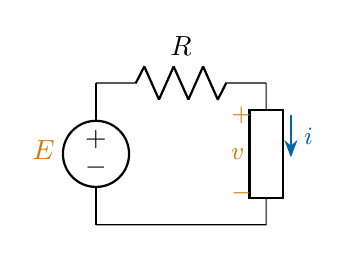
\begin{tikzpicture}[scale=0.9]
  \nlone{$\Vcol{E}$}{$R$}
\end{tikzpicture}
\end{minipage}\hfill
\begin{minipage}[c]{0.54\linewidth}
A source $E$ and a resistor $R$ drive a nonlinear resistor with the characteristic
$\Icol{i} = g(\Vcol{v})$ (a voltage-controlled resistor). KVL gives
\[
  E = R\,\Icol{i} + \Vcol{v} .
\]
The problem: find the pair $(\Vcol{v_o}, \Icol{i_o})$, the \textbf{operating point}.
\end{minipage}

\subsection{The algebraic solution}

Substitute the characteristic into KVL and solve one equation in one unknown:
\[
  E = R\,g(\Vcol{v}) + \Vcol{v} \quad\Rightarrow\quad \Vcol{v_o}, \qquad \Icol{i_o} = g(\Vcol{v_o}) .
\]
This needs a formula for $g$. Often the characteristic is only a measured curve.

\subsection{The graphical solution: the load line}

\begin{minipage}[c]{0.44\linewidth}
The pair $(\Vcol{v}, \Icol{i})$ satisfies two constraints at the same time:
\begin{itemize}
  \item the \textcolor{ccur}{circuit}: $R\,\Icol{i} + \Vcol{v} = E$, a straight line, the
        \textbf{load line};
  \item the \textcolor{metured}{element}: $\Icol{i} = g(\Vcol{v})$.
\end{itemize}
The operating point is where the two meet. The load line crosses the axes at $\Vcol{v} = E$
and $\Icol{i} = E/R$.
\end{minipage}\hfill
\begin{minipage}[c]{0.52\linewidth}
\centering
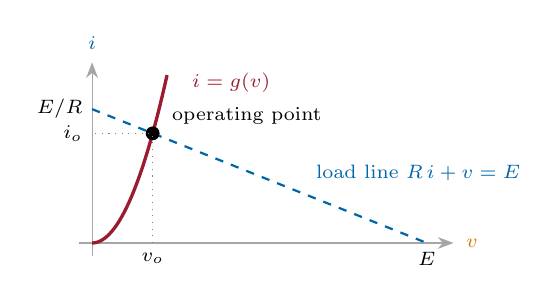
\begin{tikzpicture}[scale=0.85]
  \loadpic
\end{tikzpicture}
\end{minipage}

\bigskip
\begin{examplebox}[Example 15.1 --- the operating point]
\begin{minipage}[c]{0.44\linewidth}
\centering
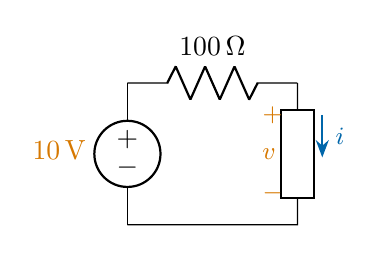
\begin{tikzpicture}[scale=0.9]
  \nlone{$\Vcol{10\V}$}{$100\ohm$}
\end{tikzpicture}
\end{minipage}\hfill
\begin{minipage}[c]{0.52\linewidth}
The nonlinear resistor has the characteristic
\[
  \Icol{i} = \begin{cases} \frac{3}{100}\,\Vcol{v}^2, & \Vcol{v} \geq 0,\\[2pt] 0, & \Vcol{v} < 0. \end{cases}
\]
Find the operating point.
\end{minipage}
\end{examplebox}

\solution

\solstep{1}{KVL}
\[
  100\,\Icol{i} + \Vcol{v} - 10 = 0 .
\]

\solstep{2}{The case $\Vcol{v} < 0$}
Here $\Icol{i} = 0$, so KVL gives $\Vcol{v} = 10\V$. This contradicts $\Vcol{v} < 0$: there is
no solution with $\Vcol{v} < 0$.

\solstep{3}{The case $\Vcol{v} \geq 0$}
\begin{minipage}[c]{0.5\linewidth}
Plug $\Icol{i} = \frac{3}{100}\,\Vcol{v}^2$ into KVL:
\begin{align*}
  3\,\Vcol{v}^2 + \Vcol{v} - 10 &= 0\\
  (3\,\Vcol{v} - 5)(\Vcol{v} + 2) &= 0 .
\end{align*}
Only $\Vcol{v} = \frac53\V$ satisfies $\Vcol{v} \geq 0$. Then
$\Icol{i} = \frac{3}{100} \cdot \frac{25}{9} = \frac{1}{12}\A$:
\[
  (\Vcol{v_o}, \Icol{i_o}) = \big(\tfrac53\V, \ \tfrac{1}{12}\A\big) .
\]
\end{minipage}\hfill
\begin{minipage}[c]{0.46\linewidth}
\centering
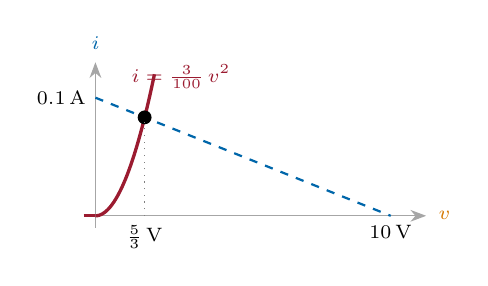
\begin{tikzpicture}[scale=0.75]
  \exOnePlot
\end{tikzpicture}
\end{minipage}

\subsection{None, one or many operating points}

\begin{minipage}[c]{0.3\linewidth}
\centering
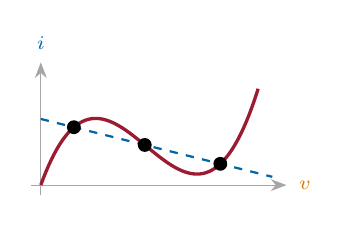
\begin{tikzpicture}[scale=0.6]
  \manypic
\end{tikzpicture}\\[2pt]
{\small many}
\end{minipage}\hfill
\begin{minipage}[c]{0.3\linewidth}
\centering
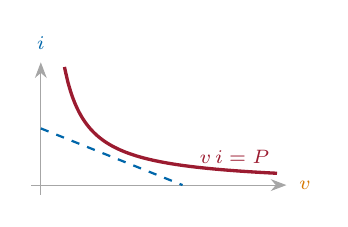
\begin{tikzpicture}[scale=0.6]
  \nonepic
\end{tikzpicture}\\[2pt]
{\small none}
\end{minipage}\hfill
\begin{minipage}[c]{0.34\linewidth}
A linear circuit with a unique solution has exactly one. A nonlinear one need not: a bent
curve can meet the load line several times, and a curve such as $\Vcol{v}\,\Icol{i} = P$ may
not meet it at all.
\end{minipage}

%==============================================================
\section{A nonlinear resistor in a larger circuit}

When the rest of the circuit is linear, three steps reduce the problem to the one of Section~1:
\begin{enumerate}
  \item find the \textbf{Th\'evenin equivalent} of the linear part, seen by the nonlinear
        resistor;
  \item find the \textbf{operating point} $(\Vcol{v_R}, \Icol{i_R})$ with the load line;
  \item by the \textbf{substitution theorem}, replace the nonlinear resistor by a voltage
        source $\Vcol{v_R}$ (or a current source $\Icol{i_R}$); no other voltage or current in
        the circuit changes, and every other variable then follows from a linear circuit.
\end{enumerate}

\medskip
\begin{examplebox}[Example 15.2 --- Th\'evenin, operating point, substitution]
\begin{minipage}[c]{0.56\linewidth}
\centering
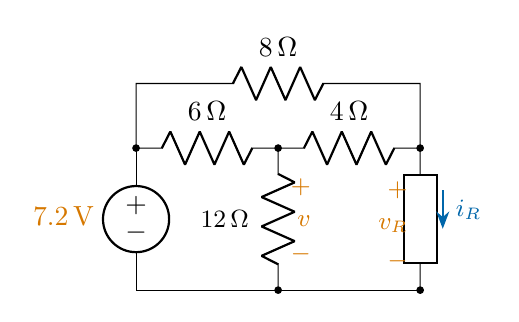
\begin{tikzpicture}[scale=0.82]
  \exTwo{0}
\end{tikzpicture}
\end{minipage}\hfill
\begin{minipage}[c]{0.4\linewidth}
The nonlinear resistor has the characteristic
\[
  \Icol{i_R} = \begin{cases} \frac14\,\Vcol{v_R}^2, & \Vcol{v_R} \geq 0,\\[2pt] 0, & \Vcol{v_R} < 0. \end{cases}
\]
Find $\Vcol{v}$.
\end{minipage}
\end{examplebox}

\solution

\solstep{1}{The Th\'evenin equivalent}
\begin{minipage}[c]{0.56\linewidth}
\centering
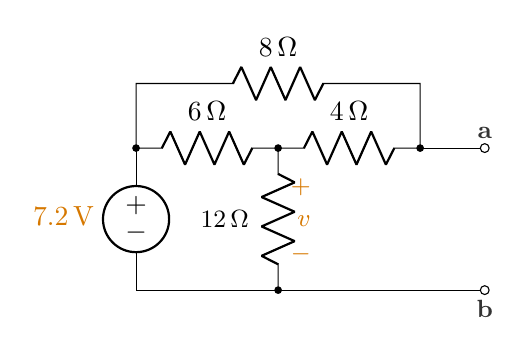
\begin{tikzpicture}[scale=0.82]
  \exTwo{1}
\end{tikzpicture}
\end{minipage}\hfill
\begin{minipage}[c]{0.4\linewidth}
Remove the nonlinear resistor; its terminals become the port a--b. Killing the $7.2\V$ source
(a short):
\[
  \Rth = 8 \parallel (4 + 6 \parallel 12) = 8 \parallel 8 = 4\ohm .
\]
\end{minipage}

\smallskip
For $\voc$, take b as the ground; with node voltages $\e{1}$ (the top of $12\ohm$) and $\e{a}$:
\begin{align*}
  \text{Node 1:}\quad & \frac{\e{1} - 7.2}{6} + \frac{\e{1}}{12} + \frac{\e{1} - \e{a}}{4} = 0\\
  \text{Node a:}\quad & \frac{\e{a} - 7.2}{8} + \frac{\e{a} - \e{1}}{4} = 0
\end{align*}
These give $\e{1} = 5.4\V$ and $\vth = \voc = \e{a} = 6\V$.

\solstep{2}{The operating point}
\begin{minipage}[c]{0.5\linewidth}
\centering
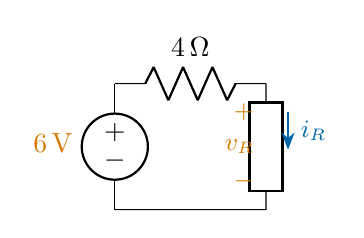
\begin{tikzpicture}[scale=0.8]
  \exTwoTh
\end{tikzpicture}\\[8pt]
KVL: \ $4\,\Icol{i_R} + \Vcol{v_R} - 6 = 0$. \ Plug
$\Icol{i_R} = \frac14\,\Vcol{v_R}^2$:
\begin{align*}
  \Vcol{v_R}^2 + \Vcol{v_R} - 6 &= 0\\
  (\Vcol{v_R} + 3)(\Vcol{v_R} - 2) &= 0 .
\end{align*}
With $\Vcol{v_R} \geq 0$: $\Vcol{v_R} = 2\V$ and $\Icol{i_R} = 1\A$.
\end{minipage}\hfill
\begin{minipage}[c]{0.46\linewidth}
\centering
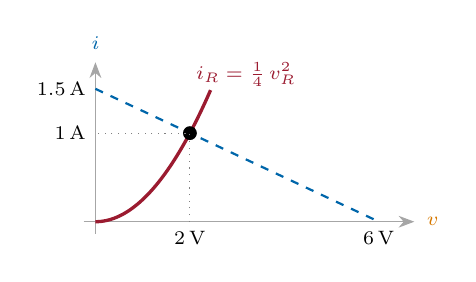
\begin{tikzpicture}[scale=0.75]
  \exTwoPlot
\end{tikzpicture}
\end{minipage}

\solstep{3}{Substitution}
\begin{minipage}[c]{0.56\linewidth}
\centering
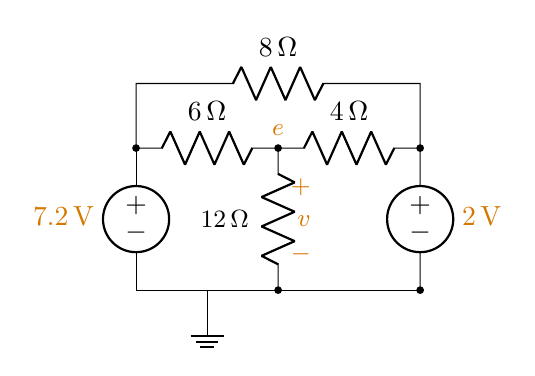
\begin{tikzpicture}[scale=0.82]
  \exTwo{2}
\end{tikzpicture}
\end{minipage}\hfill
\begin{minipage}[c]{0.4\linewidth}
Replace the nonlinear resistor by a $2\V$ source. One unknown node voltage $\e{}$ remains:
\[
  \frac{\e{} - 7.2}{6} + \frac{\e{}}{12} + \frac{\e{} - 2}{4} = 0 .
\]
\end{minipage}

\smallskip
Multiply by $12$: $\ 2\,\e{} - 14.4 + \e{} + 3\,\e{} - 6 = 0$, so
\[
  \Vcol{v} = \e{} = 3.4\V .
\]

%==============================================================
\section{The ideal diode}

\begin{definitionbox}{Ideal diode}
\begin{minipage}[c]{0.16\linewidth}
\centering
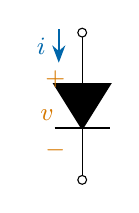
\begin{tikzpicture}[scale=0.85]
  \draw (0,2.2) to[D*] (0,0); \termtb{2.2}
\end{tikzpicture}
\end{minipage}\hfill
\begin{minipage}[c]{0.3\linewidth}
\centering
\begin{tikzpicture}[scale=0.95]
  \ivax{1.6}{1.2}{}
  \draw[crv] (-1.4,0) -- (0,0) -- (0,1.1);
  \node[font=\scriptsize, text=metured, anchor=west] at (0.05,0.85) {ON};
  \node[font=\scriptsize, text=metured, anchor=south] at (-0.8,0.05) {OFF};
\end{tikzpicture}
\end{minipage}\hfill
\begin{minipage}[c]{0.48\linewidth}
\textbf{ON:} $\Vcol{v} = 0$ and $\Icol{i} \geq 0$: a short circuit.\\[4pt]
\textbf{OFF:} $\Icol{i} = 0$ and $\Vcol{v} \leq 0$: an open circuit.\\[4pt]
The characteristic is made of two straight pieces.
\end{minipage}
\end{definitionbox}

\textbf{Turning an element around.} If the two terminals of any resistive element are swapped,
both $\Vcol{v}$ and $\Icol{i}$ change sign: the characteristic is reflected through the origin.
A reversed diode conducts for $\Icol{i} \leq 0$ and blocks for $\Vcol{v} \geq 0$.

\textbf{Series and parallel.} In series the elements carry the same current, so the voltages
add: the curves are added \emph{horizontally}. In parallel the elements share the same voltage,
so the currents add: the curves are added \emph{vertically}. Combining ideal diodes, LTI
resistors and constant sources this way always gives a \textbf{piecewise-linear}
characteristic.

\subsection{Simple series and parallel}

\newcommand{\casecell}[4]{%
  \begin{minipage}[c]{0.49\linewidth}
  \begin{minipage}[c]{0.34\linewidth}
  \centering
  \begin{tikzpicture}[scale=0.62] #1 \end{tikzpicture}
  \end{minipage}\hfill
  \begin{minipage}[c]{0.31\linewidth}
  \centering
  \begin{tikzpicture}[scale=0.66] \pframe{0}{} #2 \end{tikzpicture}
  \end{minipage}\hfill
  \begin{minipage}[c]{0.32\linewidth}
  \small\raggedright\textbf{#3}\\ #4
  \end{minipage}
  \end{minipage}}

Start with one diode and one resistor $R$. In series, the diode curve is added horizontally to
the line of $R$; in parallel, vertically.

\medskip\noindent
\casecell{\caseckta}{\caseresa}{I: $R$ and a diode in series}{$\Icol{i} > 0$: $\Vcol{v} = R\,\Icol{i}$; $\Icol{i} = 0$: $\Vcol{v} \leq 0$}\hfill
\casecell{\casecktb}{\caseresb}{II: $R$ and a diode in parallel}{$\Vcol{v} < 0$: $\Icol{i} = \Vcol{v}/R$; $\Vcol{v} = 0$: $\Icol{i} \geq 0$}

\subsection{Assume the state of the diode}

A diode is either ON (a short) or OFF (an open). With a state assumed, the circuit is linear.
The \textbf{assumed-state method}: assume a state, solve the linear circuit, and keep the result
only where the assumption holds ($\Icol{i_D} \geq 0$ for ON, $\Vcol{v_D} < 0$ for OFF).

\bigskip
\begin{examplebox}[Example 15.3 --- a diode, a resistor and a source]
\begin{minipage}[c]{0.36\linewidth}
\centering
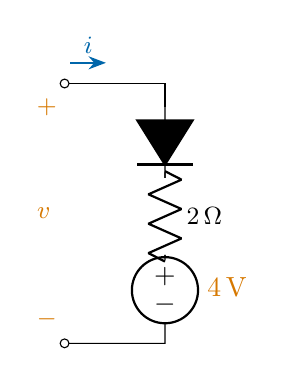
\begin{tikzpicture}[scale=0.75]
  \exS{0}
\end{tikzpicture}
\end{minipage}\hfill
\begin{minipage}[c]{0.6\linewidth}
The one-port is a diode, a $2\ohm$ resistor and a $4\V$ source in series. Find its $i$--$v$
characteristic, first by assuming states and then graphically.
\end{minipage}
\end{examplebox}

\solution

\solstep{1}{Assume the diode ON}
\begin{minipage}[c]{0.36\linewidth}
\centering
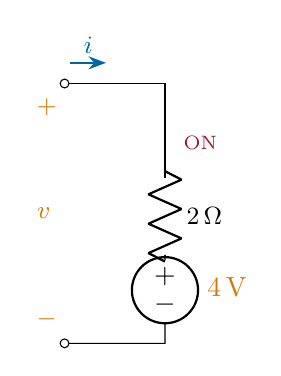
\begin{tikzpicture}[scale=0.75]
  \exS{1}
\end{tikzpicture}
\end{minipage}\hfill
\begin{minipage}[c]{0.6\linewidth}
The diode is a short. KVL:
\[
  \Vcol{v} = 2\,\Icol{i} + 4 .
\]
The diode current is $\Icol{i_D} = \Icol{i} = (\Vcol{v} - 4)/2$. The condition
$\Icol{i_D} \geq 0$ holds for $\Vcol{v} \geq 4\V$.
\end{minipage}

\solstep{2}{Assume the diode OFF}
\begin{minipage}[c]{0.36\linewidth}
\centering
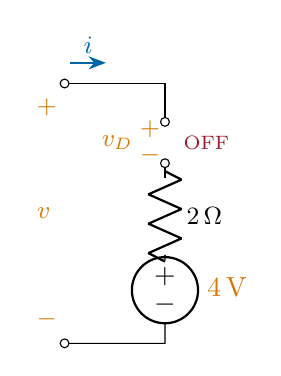
\begin{tikzpicture}[scale=0.75]
  \exS{2}
\end{tikzpicture}
\end{minipage}\hfill
\begin{minipage}[c]{0.6\linewidth}
The diode is an open, so $\Icol{i} = 0$ and the $2\ohm$ resistor has no voltage. KVL:
\[
  \Vcol{v_D} = \Vcol{v} - 4 .
\]
The condition $\Vcol{v_D} < 0$ holds for $\Vcol{v} < 4\V$.
\end{minipage}

\solstep{3}{The characteristic}
\begin{minipage}[c]{0.46\linewidth}
\[
  \Icol{i} = \begin{cases} \dfrac{\Vcol{v} - 4}{2}, & \Vcol{v} \geq 4\V,\\[10pt]
                           0, & \Vcol{v} < 4\V.\end{cases}
\]
The two ranges do not overlap and together cover every $\Vcol{v}$. The breakpoint
$(4\V, 0)$ is where $\Icol{i_D} = 0$ and $\Vcol{v_D} = 0$ at the same time.
\end{minipage}\hfill
\begin{minipage}[c]{0.5\linewidth}
\centering
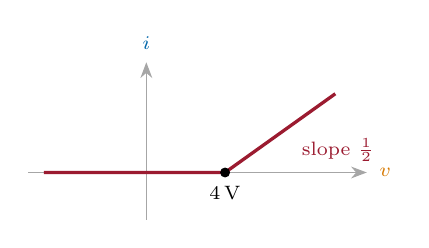
\begin{tikzpicture}[scale=1.0]
  \exSPlot
\end{tikzpicture}
\end{minipage}

\solstep{4}{Graphically}
\begin{center}
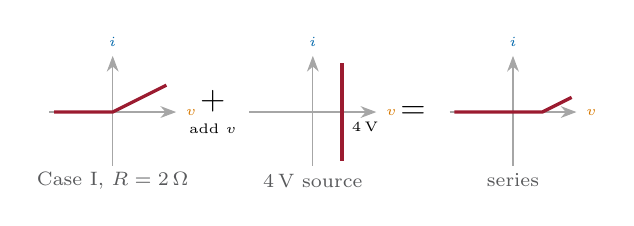
\begin{tikzpicture}[scale=0.62]
  \threeplots{\draw[crv] (-1.2,0) -- (0,0) -- (1.1,0.55);}{\draw[crv] (0.6,-1.0) -- (0.6,1.0); \node[font=\tiny, below right] at (0.6,0) {$4\V$};}{\draw[crv] (-1.2,0) -- (0.6,0) -- (1.2,0.3);}{\shortstack{$+$\\[1pt]{\tiny add $v$}}}{Case I, $R = 2\ohm$}{$4\V$ source}{series}
\end{tikzpicture}
\end{center}
The diode and $2\ohm$ are Case I. The source is a vertical line at $\Vcol{v} = 4\V$; adding it
horizontally shifts the curve right by $4\V$: the same result. \ \yes

\subsection{More connections}

The same reasoning gives the characteristics of the connections below. In each one, find the
piece with the diode ON, the piece with it OFF, and the breakpoint.

\medskip\noindent
\casecell{\casecktc}{\caseresc}{III: reversed diode $\parallel R_1$, then $R_2$}{slope $\frac{1}{R_1 + R_2}$ for $\Icol{i} > 0$, $\frac{1}{R_2}$ for $\Icol{i} < 0$}\hfill
\casecell{\casecktd}{\caseresd}{IV: diode and $R_1$, in parallel with $R_2$}{slope $\frac{1}{R_1} + \frac{1}{R_2}$ for $\Vcol{v} > 0$, $\frac{1}{R_2}$ for $\Vcol{v} < 0$}

\medskip\noindent
\casecell{\caseckte}{\caserese}{V: a diode and a source $E$ in series}{the diode curve shifted right by $E$}\hfill
\casecell{\casecktf}{\caseresf}{VI: a diode and a source $I$ in parallel}{the diode curve shifted up by $I$}

\medskip\noindent
\casecell{\casecktg}{\caseresg}{VII: Case VI in series with $E$ ($+$ at the bottom)}{Case VI shifted left by $E$}\hfill
\begin{minipage}[c]{0.49\linewidth}
\small A voltage source in series shifts a curve horizontally; a current source in parallel
shifts it vertically.
\end{minipage}

\subsection{The ideal Zener diode}

\begin{minipage}[c]{0.14\linewidth}
\centering
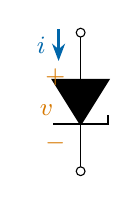
\begin{tikzpicture}[scale=0.8]
  \draw (0,2.2) to[zD*] (0,0); \termtb{2.2}
\end{tikzpicture}
\end{minipage}\hfill
\begin{minipage}[c]{0.3\linewidth}
\centering
\begin{tikzpicture}[scale=0.9]
  \zenerPlot
\end{tikzpicture}
\end{minipage}\hfill
\begin{minipage}[c]{0.2\linewidth}
\centering
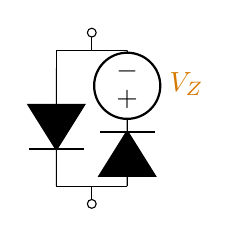
\begin{tikzpicture}[scale=0.75]
  \zenerEq
\end{tikzpicture}
\end{minipage}\hfill
\begin{minipage}[c]{0.32\linewidth}
In the forward direction the Zener diode is an ideal diode. In the reverse direction it blocks
until $\Vcol{v} = -V_Z$, and then holds that voltage. It is equivalent to a diode in parallel
with a reversed diode and a battery $V_Z$ in series.
\end{minipage}

%==============================================================
\section{Piecewise-linear circuits}

\subsection{The characteristic of a circuit}

With $n$ diodes there are $2^n$ combinations of states, and each gives a linear circuit. Solve
each one, keep it where its conditions hold, and drop the impossible ones. Each diode adds at
most one breakpoint.

\bigskip
\begin{examplebox}[Example 15.4 --- two diodes]
\begin{minipage}[c]{0.44\linewidth}
\centering
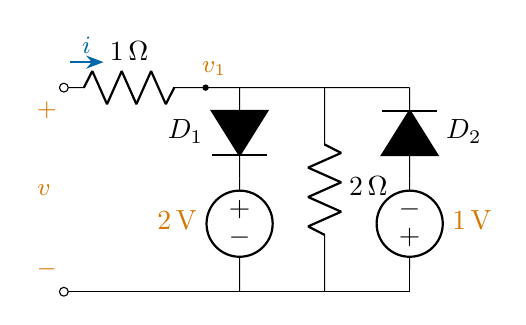
\begin{tikzpicture}[scale=0.72]
  \exH
\end{tikzpicture}
\end{minipage}\hfill
\begin{minipage}[c]{0.52\linewidth}
A $1\ohm$ resistor is in series with three parallel branches: $D_1$ with a $2\V$ source, a
$2\ohm$ resistor, and a reversed $D_2$ with a $1\V$ source. $\Vcol{v_1}$ is the voltage of the
parallel part. Find the $i$--$v$ characteristic of the one-port.
\end{minipage}
\end{examplebox}

\solution

\solstep{1}{Both diodes OFF}
Only the $1\ohm$ and $2\ohm$ resistors carry current, in series:
\[
  \Vcol{v_1} = 2\,\Icol{i}, \qquad \Vcol{v} = 3\,\Icol{i} .
\]
The diode voltages are $\Vcol{v_{D_1}} = \Vcol{v_1} - 2$ and $\Vcol{v_{D_2}} = -1 - \Vcol{v_1}$.
Both are negative for $-1 < \Vcol{v_1} < 2$, that is $-0.5 < \Icol{i} < 1$, or
$-1.5\V < \Vcol{v} < 3\V$.

\solstep{2}{$D_1$ ON, $D_2$ OFF}
$D_1$ is a short, so $\Vcol{v_1} = 2\V$ and
\[
  \Vcol{v} = \Icol{i} + 2 .
\]
The $2\ohm$ resistor carries $1\A$, so $\Icol{i_{D_1}} = \Icol{i} - 1$. The condition
$\Icol{i_{D_1}} \geq 0$ holds for $\Icol{i} \geq 1$, or $\Vcol{v} \geq 3\V$. Check $D_2$:
$\Vcol{v_{D_2}} = -1 - 2 < 0$. \ \yes

\solstep{3}{$D_2$ ON, $D_1$ OFF}
$D_2$ is a short, so $\Vcol{v_1} = -1\V$ and
\[
  \Vcol{v} = \Icol{i} - 1 .
\]
The $2\ohm$ resistor carries $-0.5\A$. KCL at the top node gives the forward current of $D_2$
(upward): $\Icol{i_{D_2}} = -0.5 - \Icol{i}$. The condition $\Icol{i_{D_2}} \geq 0$ holds for
$\Icol{i} \leq -0.5$, or $\Vcol{v} \leq -1.5\V$. Check $D_1$: $\Vcol{v_{D_1}} = -1 - 2 < 0$. \ \yes

\solstep{4}{Both diodes ON}
This would need $\Vcol{v_1} = 2$ and $\Vcol{v_1} = -1$ at the same time: impossible.

\solstep{5}{The characteristic}
\begin{minipage}[c]{0.5\linewidth}
\[
  \Icol{i} = \begin{cases} \Vcol{v} - 2, & \Vcol{v} \geq 3\V,\\[4pt]
                           \Vcol{v}/3, & -1.5\V \leq \Vcol{v} \leq 3\V,\\[4pt]
                           \Vcol{v} + 1, & \Vcol{v} \leq -1.5\V.\end{cases}
\]
{\raggedright Two diodes give two breakpoints:\\ $(-1.5\V, -0.5\A)$ and $(3\V, 1\A)$.\par}
\end{minipage}\hfill
\begin{minipage}[c]{0.46\linewidth}
\centering
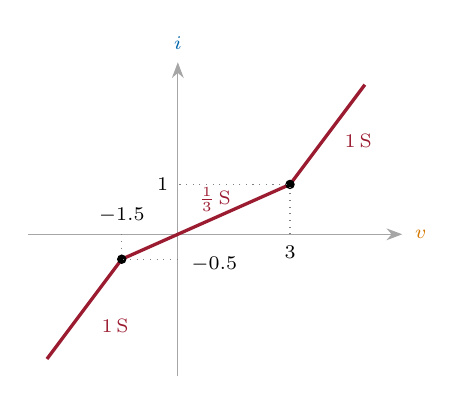
\begin{tikzpicture}[scale=0.95]
  \exHPlot
\end{tikzpicture}
\end{minipage}

\solstep{6}{Graphically}
\begin{center}
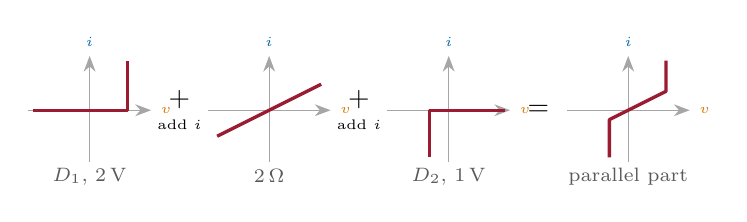
\begin{tikzpicture}[scale=0.6]
  \begin{scope}\pframe{0}{$D_1$, $2\V$} \draw[crv] (-1.2,0) -- (0.8,0) -- (0.8,1.05); \end{scope}
  \node at (1.9,0) {\shortstack{$+$\\[1pt]{\tiny add $i$}}};
  \begin{scope}[xshift=3.8cm]\pframe{0}{$2\ohm$} \draw[crv] (-1.1,-0.55) -- (1.1,0.55); \end{scope}
  \node at (5.7,0) {\shortstack{$+$\\[1pt]{\tiny add $i$}}};
  \begin{scope}[xshift=7.6cm]\pframe{0}{$D_2$, $1\V$} \draw[crv] (-0.4,-1.0) -- (-0.4,0) -- (1.2,0); \end{scope}
  \node at (9.5,0) {$=$};
  \begin{scope}[xshift=11.4cm]\pframe{0}{parallel part} \draw[crv] (-0.4,-1.0) -- (-0.4,-0.2) -- (0.8,0.4) -- (0.8,1.05); \end{scope}
\end{tikzpicture}\\[10pt]
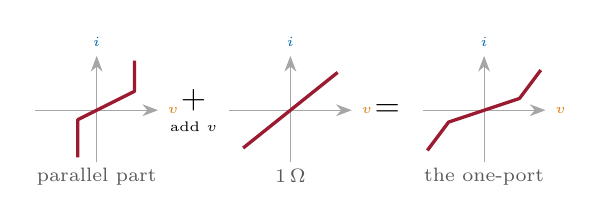
\begin{tikzpicture}[scale=0.6]
  \threeplots{\draw[crv] (-0.4,-1.0) -- (-0.4,-0.2) -- (0.8,0.4) -- (0.8,1.05);}{\pR{1.0}}{\draw[crv] (-1.2,-0.85) -- (-0.75,-0.25) -- (0.75,0.25) -- (1.2,0.85);}{\shortstack{$+$\\[1pt]{\tiny add $v$}}}{parallel part}{$1\ohm$}{the one-port}
\end{tikzpicture}
\end{center}
The first branch is Case V: vertical at $\Vcol{v_1} = 2\V$. The third is Case V turned around:
vertical at $\Vcol{v_1} = -1\V$. Adding the three currents gives the parallel part: slope
$\frac12$ between the two vertical pieces. Adding the $1\ohm$ horizontally turns the slopes
into $\frac{1}{1 + 2} = \frac13$ in the middle and $1$ outside. \ \yes

\subsection{A circuit from a characteristic}

The reverse problem: given a piecewise-linear characteristic, find a circuit. Split the curve
into pieces whose circuits are known (the basic connections above), using horizontal addition
(series) or vertical addition (parallel), and connect the pieces. Each breakpoint needs a
diode. The answer is \textbf{not unique}: different circuits can have the same characteristic.

\bigskip
\begin{examplebox}[Example 15.5 --- one breakpoint]
\begin{minipage}[c]{0.44\linewidth}
\centering
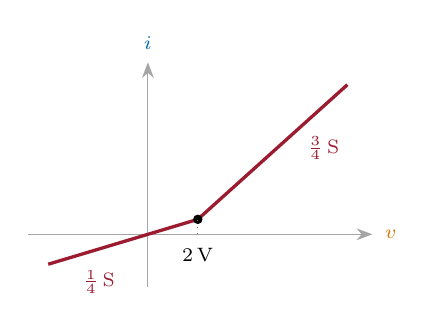
\begin{tikzpicture}[scale=0.95]
  \synPlot
\end{tikzpicture}
\end{minipage}\hfill
\begin{minipage}[c]{0.52\linewidth}
The characteristic is $\Icol{i} = \Vcol{v}/4$ for $\Vcol{v} \leq 2\V$ and has slope
$\frac34\Sie$ for $\Vcol{v} \geq 2\V$. Find a circuit with this characteristic.
\end{minipage}
\end{examplebox}

\solution

\solstep{1}{Count the breakpoints}
There is one breakpoint, at $(2\V, 0.5\A)$, so one diode is enough. Below it the curve is a line
through the origin with slope $\frac14\Sie$: a $4\ohm$ resistor.

\solstep{2}{Split it in parallel (add currents)}
\begin{center}
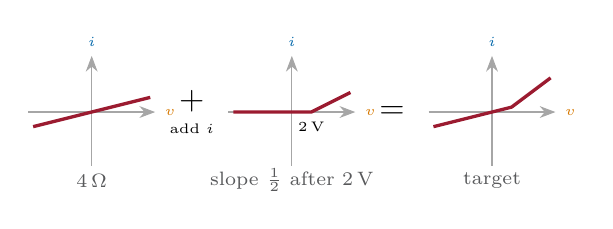
\begin{tikzpicture}[scale=0.62]
  \threeplots{\draw[crv] (-1.2,-0.3) -- (1.2,0.3);}{\draw[crv] (-1.2,0) -- (0.4,0) -- (1.2,0.4); \node[font=\tiny, below] at (0.4,0) {$2\V$};}{\draw[crv] (-1.2,-0.3) -- (0.4,0.1) -- (1.2,0.7);}{\shortstack{$+$\\[1pt]{\tiny add $i$}}}{$4\ohm$}{slope $\frac12$ after $2\V$}{target}
\end{tikzpicture}
\end{center}
Keep the $4\ohm$ resistor for all $\Vcol{v}$. Above $2\V$ the slope must grow by
$\frac34 - \frac14 = \frac12\Sie$. A branch with zero current below $2\V$ and slope $\frac12\Sie$
above is Case I with $R = 2\ohm$, shifted right by a $2\V$ source in series. Since the currents
add, this branch goes in parallel with the $4\ohm$ resistor.

\solstep{3}{The circuit}
\begin{minipage}[c]{0.36\linewidth}
\centering
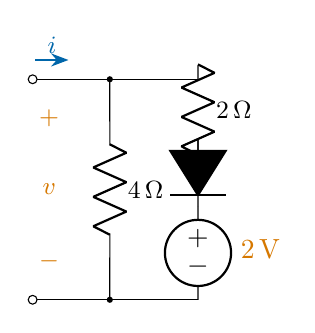
\begin{tikzpicture}[scale=0.7]
  \synCkt
\end{tikzpicture}
\end{minipage}\hfill
\begin{minipage}[c]{0.6\linewidth}
A $4\ohm$ resistor in parallel with a branch of $2\ohm$, a diode and a $2\V$ source. Check at
$\Vcol{v} = 4\V$: the resistor carries $1\A$ and the branch $(4 - 2)/2 = 1\A$, so
$\Icol{i} = 2\A$; the target gives $0.5 + \frac34 \cdot 2 = 2\A$. \ \yes \ The elements of the
branch can be put in any order: the circuit is not unique.
\end{minipage}

The next example needs two diodes and both kinds of addition.

\bigskip
\begin{examplebox}[Example 15.6 --- a circuit with two breakpoints]
\begin{minipage}[c]{0.44\linewidth}
\centering
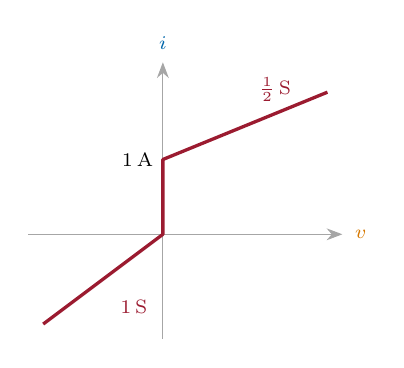
\begin{tikzpicture}[scale=0.95]
  \exFourPlot
\end{tikzpicture}
\end{minipage}\hfill
\begin{minipage}[c]{0.52\linewidth}
The characteristic has slope $1\Sie$ for $\Vcol{v} < 0$, a vertical piece from $0$ to $1\A$
at $\Vcol{v} = 0$, and slope $\frac12\Sie$ above $1\A$. Find a circuit with this
characteristic.
\end{minipage}
\end{examplebox}

\needspace{12\baselineskip}
\solution

\solstep{1}{Split it in series (add voltages)}
\begin{center}
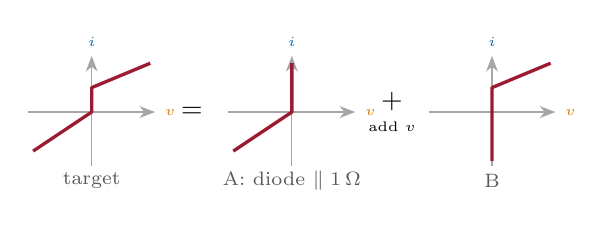
\begin{tikzpicture}[scale=0.62]
  \begin{scope}\pframe{0}{target} \draw[crv] (-1.2,-0.8) -- (0,0) -- (0,0.5) -- (1.2,1.0); \end{scope}
  \node at (2.05,0) {$=$};
  \begin{scope}[xshift=4.1cm]\pframe{0}{A: diode $\parallel 1\ohm$} \draw[crv] (-1.2,-0.8) -- (0,0) -- (0,1.0); \end{scope}
  \node at (6.15,0) {\shortstack{$+$\\[1pt]{\tiny add $v$}}};
  \begin{scope}[xshift=8.2cm]\pframe{0}{B} \draw[crv] (0,-1.0) -- (0,0.5) -- (1.2,1.0); \end{scope}
\end{tikzpicture}
\end{center}
Piece A is Case II with $R = 1\ohm$: it gives the slope $1\Sie$ for $\Vcol{v} < 0$ and is a
short for $\Icol{i} \geq 0$. Piece B is a short for $\Icol{i} \leq 1\A$ and has slope
$\frac12\Sie$ above $1\A$.

\solstep{2}{Split B in parallel (add currents)}
\begin{center}
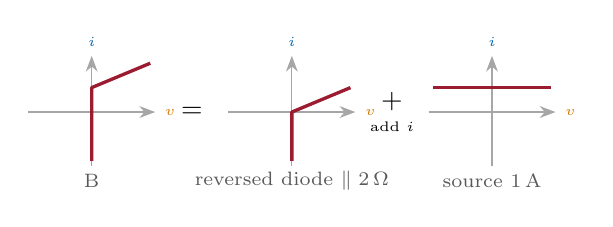
\begin{tikzpicture}[scale=0.62]
  \begin{scope}\pframe{0}{B} \draw[crv] (0,-1.0) -- (0,0.5) -- (1.2,1.0); \end{scope}
  \node at (2.05,0) {$=$};
  \begin{scope}[xshift=4.1cm]\pframe{0}{reversed diode $\parallel 2\ohm$} \draw[crv] (0,-1.0) -- (0,0) -- (1.2,0.5); \end{scope}
  \node at (6.15,0) {\shortstack{$+$\\[1pt]{\tiny add $i$}}};
  \begin{scope}[xshift=8.2cm]\pframe{0}{source $1\A$} \draw[crv] (-1.2,0.5) -- (1.2,0.5); \end{scope}
\end{tikzpicture}
\end{center}
A reversed diode in parallel with $2\ohm$ is Case II reflected through the origin. A $1\A$
current source in parallel lifts it by $1\A$ (Case VI).

\solstep{3}{The circuit}
\begin{minipage}[c]{0.36\linewidth}
\centering
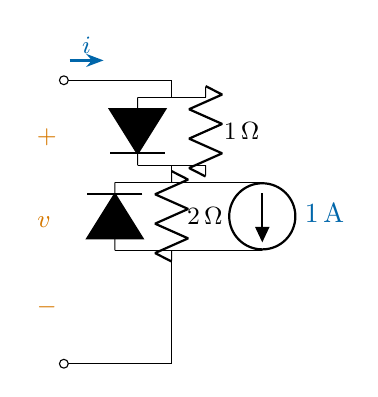
\begin{tikzpicture}[scale=0.72]
  \exFourCkt
\end{tikzpicture}
\end{minipage}\hfill
\begin{minipage}[c]{0.6\linewidth}
Piece A (a diode in parallel with $1\ohm$) in series with piece B (a reversed diode, $2\ohm$
and the $1\A$ source, all in parallel). Check at $\Vcol{v} = 2\V$: the top diode is ON (a
short), the bottom diode is OFF, and $\Icol{i} = 1 + 2/2 = 2\A$. \ \yes
\end{minipage}

\bigskip
\begin{examplebox}[Example 15.7 --- a numerical characteristic]
\begin{minipage}[c]{0.44\linewidth}
\centering
\begin{tikzpicture}[scale=0.95]
  \exFivePlot
\end{tikzpicture}
\end{minipage}\hfill
\begin{minipage}[c]{0.52\linewidth}
The characteristic passes through the origin with slope $1\Sie$ for
$-2\V < \Vcol{v} < 2\V$ and slope $2\Sie$ outside this interval. Find a circuit.
\end{minipage}
\end{examplebox}

\solution

\solstep{1}{Split it in parallel (add currents)}
All pieces share the voltage $\Vcol{v}$, so write the current as a sum:
\begin{itemize}
  \item a $1\ohm$ resistor: the slope $1\Sie$ in the middle;
  \item a branch with current $\Vcol{v} - 2$ for $\Vcol{v} > 2\V$ and zero otherwise;
  \item a branch with current $\Vcol{v} + 2$ for $\Vcol{v} < -2\V$ and zero otherwise.
\end{itemize}
Outside $\pm 2\V$ one branch adds $1\Sie$, so the slope becomes $2\Sie$.

\solstep{2}{The two branches}
The second piece is like the branch of Example 15.5, now with $1\ohm$: a resistor, a diode and a
$2\V$ source in series, conducting only when $\Vcol{v} > 2\V$. The third piece is its
reflection through the origin: the same branch turned around.

\solstep{3}{The circuit}
\begin{minipage}[c]{0.56\linewidth}
\centering
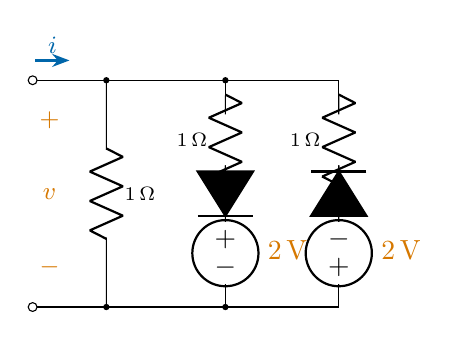
\begin{tikzpicture}[scale=0.72]
  \exFiveCkt
\end{tikzpicture}
\end{minipage}\hfill
\begin{minipage}[c]{0.4\linewidth}
Check at $\Vcol{v} = 3\V$: the resistor carries $3\A$, the middle branch $3 - 2 = 1\A$ and
the reversed branch $0$; in total $4\A$. The target gives $2 + 2 \cdot 1 = 4\A$. \ \yes
\end{minipage}

%==============================================================
\section{Linear time-varying circuits}

A linear time-varying (LTV) resistor has the characteristic $\Vcol{v} = R(t)\,\Icol{i}$: at each
instant a line through the origin, but its slope changes with time. Such circuits are not
nonlinear, and at each instant they are solved like LTI circuits.

\medskip
\begin{examplebox}[Example 15.8 --- a linear time-varying circuit]
\begin{minipage}[c]{0.52\linewidth}
\centering
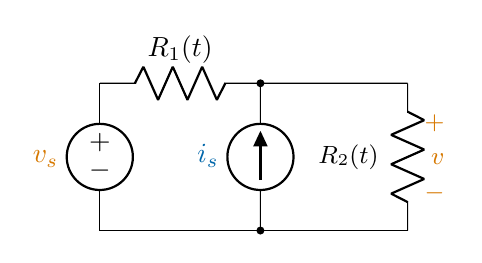
\begin{tikzpicture}[scale=0.85]
  \exSix
\end{tikzpicture}
\end{minipage}\hfill
\begin{minipage}[c]{0.44\linewidth}
$R_1(t)$ and $R_2(t)$ are linear time-varying resistors. Express $\Vcol{v}$ in terms of the
inputs $\Vcol{v_s}$ and $\Icol{i_s}$. Does superposition still hold?
\end{minipage}
\end{examplebox}

\solution

\solstep{1}{KCL at the top node}
\[
  \frac{\Vcol{v} - \Vcol{v_s}}{R_1(t)} - \Icol{i_s} + \frac{\Vcol{v}}{R_2(t)} = 0 .
\]

\solstep{2}{Solve for $\Vcol{v}$}
\[
  \Vcol{v} = \underbrace{\frac{R_2(t)}{R_1(t) + R_2(t)}}_{k_1(t)}\,\Vcol{v_s}
  + \underbrace{\frac{R_1(t)\,R_2(t)}{R_1(t) + R_2(t)}}_{k_2(t)}\,\Icol{i_s}
  = \mathbf{k}(t)\,\mathbf{u} ,
\]
with the input vector $\mathbf{u} = [\,\Vcol{v_s}\ \ \Icol{i_s}\,]^{\mathsf T}$ and
$\mathbf{k}(t) = [\,k_1(t)\ \ k_2(t)\,]$.

\solstep{3}{Superposition}
For input vectors $\mathbf{u}$, $\mathbf{w}$ and numbers $\alpha$, $\beta$,
$\Vcol{v}(\alpha\,\mathbf{u} + \beta\,\mathbf{w}) = \alpha\,\Vcol{v}(\mathbf{u}) +
\beta\,\Vcol{v}(\mathbf{w})$: superposition still holds for LTV resistive circuits. Only the
coefficients $k_1$, $k_2$ now depend on time.

\needspace{14\baselineskip}
%==============================================================
\section*{Summary}

\begin{center}
\small
\renewcommand{\arraystretch}{1.3}
\begin{tabular}{@{}>{\raggedright}p{4.4cm} >{\raggedright\arraybackslash}p{11.3cm}@{}}
\toprule
\textbf{In the circuit} & \textbf{What to do}\\
\midrule
one nonlinear resistor & solve $E = R\,g(\Vcol{v}) + \Vcol{v}$, or intersect the load line $R\,\Icol{i} + \Vcol{v} = E$ with $\Icol{i} = g(\Vcol{v})$\\
a linear rest & Th\'evenin equivalent, operating point, then the substitution theorem\\
ideal diodes & assume ON ($\Vcol{v_D} = 0$, $\Icol{i_D} \geq 0$) or OFF ($\Icol{i_D} = 0$, $\Vcol{v_D} < 0$), solve, check\\
series, parallel connections & add the curves horizontally (voltages) or vertically (currents)\\
a given characteristic & split it into known pieces; each breakpoint needs a diode; not unique\\
linear time-varying resistors & $\Vcol{v} = \mathbf{k}(t)\,\mathbf{u}$: superposition still holds\\
\bottomrule
\end{tabular}
\end{center}

\end{document}
